% \textbf{\underline{OZ 2 - Magnetische velden - Oefening 5:}}
% \vspace{0.5cm}

% Een soort "projectile launcher" wordt getoond op Figuur 2.2. Een grootte stroom vloeit in een gesloten lus samengesteld uit rails, een spanningsbron en een zeer lichte weerstandsloze bar die over de rails ligt. Een 1,8 T magnetisch veld staat loodrecht op het vlak van het circuit. Indien de rails een afstand $ d = 24 $ cm gescheiden zijn, en de bar een massa van 1,5 g heeft, welke constante stroom is nodig om de bar vanuit rust te versnellen tot 25 m/s in een afstand van 1,0 m? Wat is de zin van het magneetveld?

% \begin{figure}[H]
%     \centering
%     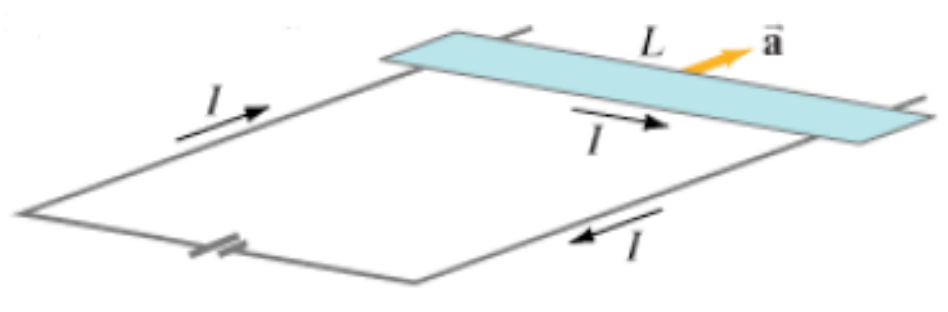
\includegraphics[width=6cm]{oz02/resources/oef-5-opgave.png}
    
%     \textbf{Figuur 2.2}
% \end{figure}

% \begin{description}[labelwidth=1.5cm, leftmargin=!]
%     \item[Geg. :]   $ B = 1,8 $ T; $ d = 24 $ cm; $ m = 1,5 $ g; $ v_0 = 0 $ m/s; $ v_e = 25 $ m/s; $ s_0 = 0 $ m; $ s_e = 1,0 $ m;
%     \item[Gevr. :]  $ I $; zin van $ \vec{B} $;
%     \item[Opl. :]   De zin van het magneetveld is naar onder gericht (In het blad). (Linkerhandregel van Fleming)
                    
%                     $ v(t) = v_0 + a t = a t $
                    
%                     $ s(t) = s_0 + v_0 t + \dfrac{a t^2}{2} = \dfrac{a t^2}{2} = \dfrac{v(t) t}{2} $
                    
%                     \hspace{-0.57 cm} $ \Leftrightarrow 
%                     s_e = \dfrac{v_e t_e}{2} $
                    
%                     \hspace{-0.57 cm} $ \Leftrightarrow 
%                     t_e = \dfrac{2 s_e}{v_e} 
%                     = \dfrac{2 \cdot 1,0}{25} 
%                     = 0,08 $ s
                    
%                     $ v(t) = a t $
                    
%                     \hspace{-0.57 cm} $ \Leftrightarrow 
%                     a = \dfrac{v_e}{t_e} 
%                     = \dfrac{25}{0,08} 
%                     = 312,5 $ m/s$ ^2 $
    
%                     $ d\vec{F} = I d\vec{s} \times \vec{B} $
                    
%                     \hspace{-0.57 cm} $ \Leftrightarrow 
%                     dF = I ds B $ \hspace{3.5cm} $ (\theta = 90^{\circ} \Rightarrow \sin{\theta} = 1) $
                    
%                     $ F = \int_{0}^{d}{I B ds}
%                     = \left[ I B s \right]_{0}^{d} = I B d $
                    
%                     $ F = m a $
                    
%                     \hspace{-0.57 cm} $ \Leftrightarrow 
%                     I B d = m a $
                    
%                     \hspace{-0.57 cm} $ \Leftrightarrow 
%                     I = \dfrac{m a}{B d} 
%                     = \dfrac{1,5 \cdot 10^{-3} \cdot 312,5}{1,8 \cdot 24 \cdot 10^{-2}} 
%                     = 1,08506944... $ A
%                     $ \approx 1,1 $ A
                    
                    
% \end{description}

% \vspace{1cm}